\chapter{Đường đi và chu trình}

\index{path!Eulerian}
\index{đường đi!Euler}
\index{path!Hamiltonian}
\index{đường đi!Hamilton}
\index{circuit!Eulerian}
\index{chu trình!Euler}
\index{circuit!Hamiltonian}
\index{chu trình!Hamilton}

Chương này tập trung vào hai loại đường đi trong đồ thị:
\begin{itemize}
\item Một \key{đường đi Euler} là một đường đi
đi qua mỗi cạnh đúng một lần.
\item Một \key{đường đi Hamilton} là một đường đi
thăm mỗi đỉnh đúng một lần.
\end{itemize}

Mặc dù đường đi Euler và Hamilton trông giống như
các khái niệm tương tự thoạt nhìn,
các bài toán tính toán liên quan đến chúng
rất khác nhau.
Hóa ra có một quy tắc đơn giản
xác định xem một đồ thị có chứa đường đi Euler hay không,
và cũng có một thuật toán hiệu quả để
tìm một đường đi như vậy nếu nó tồn tại.
Ngược lại, việc kiểm tra sự tồn tại của một đường đi Hamilton là một bài toán NP-khó, và không có thuật toán hiệu quả nào được biết để giải quyết bài toán này.

\section{Đường đi Euler}

\index{Eulerian path}
\index{đường đi Euler}

Một \key{đường đi Euler}\footnote{L. Euler đã nghiên cứu những đường đi như vậy vào năm 1736
khi ông giải quyết bài toán bảy cây cầu nổi tiếng ở Königsberg.
Đây là sự ra đời của lý thuyết đồ thị.} là một đường đi
đi qua đúng một lần qua mỗi cạnh của đồ thị.
Ví dụ, đồ thị
\begin{center}
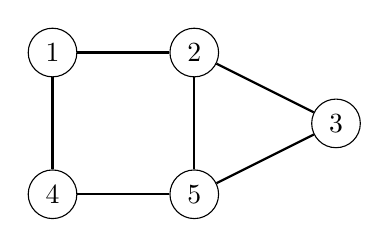
\begin{tikzpicture}[scale=0.9]
\node[draw, circle] (1) at (1,5) {$1$};
\node[draw, circle] (2) at (3,5) {$2$};
\node[draw, circle] (3) at (5,4) {$3$};
\node[draw, circle] (4) at (1,3) {$4$};
\node[draw, circle] (5) at (3,3) {$5$};

\path[draw,thick,-] (1) -- (2);
\path[draw,thick,-] (2) -- (3);
\path[draw,thick,-] (1) -- (4);
\path[draw,thick,-] (3) -- (5);
\path[draw,thick,-] (2) -- (5);
\path[draw,thick,-] (4) -- (5);
\end{tikzpicture}
\end{center}
có một đường đi Euler từ đỉnh 2 đến đỉnh 5:
\begin{center}
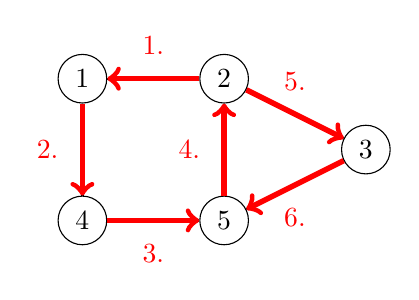
\begin{tikzpicture}[scale=0.9]
\node[draw, circle] (1) at (1,5) {$1$};
\node[draw, circle] (2) at (3,5) {$2$};
\node[draw, circle] (3) at (5,4) {$3$};
\node[draw, circle] (4) at (1,3) {$4$};
\node[draw, circle] (5) at (3,3) {$5$};

\path[draw,thick,-] (1) -- (2);
\path[draw,thick,-] (2) -- (3);
\path[draw,thick,-] (1) -- (4);
\path[draw,thick,-] (3) -- (5);
\path[draw,thick,-] (2) -- (5);
\path[draw,thick,-] (4) -- (5);

\path[draw=red,thick,->,line width=2pt] (2) -- node[font=\small,label={[red]north:1.}] {} (1);
\path[draw=red,thick,->,line width=2pt] (1) -- node[font=\small,label={[red]left:2.}] {} (4);
\path[draw=red,thick,->,line width=2pt] (4) -- node[font=\small,label={[red]south:3.}] {} (5);
\path[draw=red,thick,->,line width=2pt] (5) -- node[font=\small,label={[red]left:4.}] {} (2);
\path[draw=red,thick,->,line width=2pt] (2) -- node[font=\small,label={[red]north:5.}] {} (3);
\path[draw=red,thick,->,line width=2pt] (3) -- node[font=\small,label={[red]south:6.}] {} (5);
\end{tikzpicture}
\end{center}
\index{Eulerian circuit}
\index{chu trình Euler}
Một \key{chu trình Euler}
là một đường đi Euler bắt đầu và kết thúc
tại cùng một đỉnh.
Ví dụ, đồ thị
\begin{center}
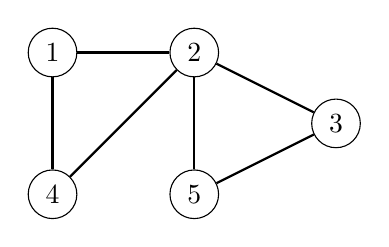
\begin{tikzpicture}[scale=0.9]
\node[draw, circle] (1) at (1,5) {$1$};
\node[draw, circle] (2) at (3,5) {$2$};
\node[draw, circle] (3) at (5,4) {$3$};
\node[draw, circle] (4) at (1,3) {$4$};
\node[draw, circle] (5) at (3,3) {$5$};

\path[draw,thick,-] (1) -- (2);
\path[draw,thick,-] (2) -- (3);
\path[draw,thick,-] (1) -- (4);
\path[draw,thick,-] (3) -- (5);
\path[draw,thick,-] (2) -- (5);
\path[draw,thick,-] (2) -- (4);
\end{tikzpicture}
\end{center}
có một chu trình Euler bắt đầu và kết thúc tại đỉnh 1:
\begin{center}
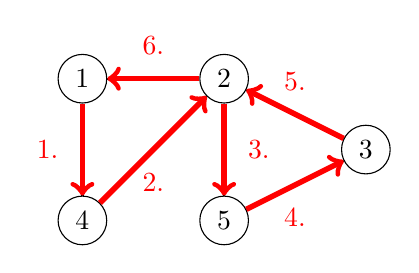
\begin{tikzpicture}[scale=0.9]
\node[draw, circle] (1) at (1,5) {$1$};
\node[draw, circle] (2) at (3,5) {$2$};
\node[draw, circle] (3) at (5,4) {$3$};
\node[draw, circle] (4) at (1,3) {$4$};
\node[draw, circle] (5) at (3,3) {$5$};

\path[draw,thick,-] (1) -- (2);
\path[draw,thick,-] (2) -- (3);
\path[draw,thick,-] (1) -- (4);
\path[draw,thick,-] (3) -- (5);
\path[draw,thick,-] (2) -- (5);
\path[draw,thick,-] (2) -- (4);

\path[draw=red,thick,->,line width=2pt] (1) -- node[font=\small,label={[red]left:1.}] {} (4);
\path[draw=red,thick,->,line width=2pt] (4) -- node[font=\small,label={[red]south:2.}] {} (2);
\path[draw=red,thick,->,line width=2pt] (2) -- node[font=\small,label={[red]right:3.}] {} (5);
\path[draw=red,thick,->,line width=2pt] (5) -- node[font=\small,label={[red]south:4.}] {} (3);
\path[draw=red,thick,->,line width=2pt] (3) -- node[font=\small,label={[red]north:5.}] {} (2);
\path[draw=red,thick,->,line width=2pt] (2) -- node[font=\small,label={[red]north:6.}] {} (1);
\end{tikzpicture}
\end{center}

\subsubsection{Sự tồn tại}

Sự tồn tại của đường đi và chu trình Euler
phụ thuộc vào bậc của các đỉnh.
Đầu tiên, một đồ thị vô hướng có một đường đi Euler
chính xác khi tất cả các cạnh
thuộc cùng một thành phần liên thông và
\begin{itemize}
\item bậc của mỗi đỉnh là chẵn \emph{hoặc}
\item bậc của đúng hai đỉnh là lẻ,
và bậc của tất cả các đỉnh khác là chẵn.
\end{itemize}

Trong trường hợp đầu tiên, mỗi đường đi Euler cũng là một chu trình Euler.
Trong trường hợp thứ hai, các đỉnh bậc lẻ là các đỉnh bắt đầu
và kết thúc của một đường đi Euler không phải là một chu trình Euler.

\begin{samepage}
Ví dụ, trong đồ thị
\begin{center}
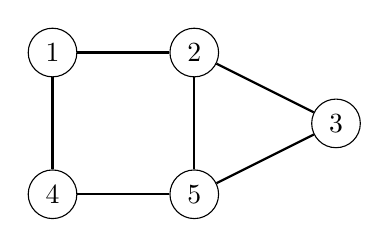
\begin{tikzpicture}[scale=0.9]
\node[draw, circle] (1) at (1,5) {$1$};
\node[draw, circle] (2) at (3,5) {$2$};
\node[draw, circle] (3) at (5,4) {$3$};
\node[draw, circle] (4) at (1,3) {$4$};
\node[draw, circle] (5) at (3,3) {$5$};

\path[draw,thick,-] (1) -- (2);
\path[draw,thick,-] (2) -- (3);
\path[draw,thick,-] (1) -- (4);
\path[draw,thick,-] (3) -- (5);
\path[draw,thick,-] (2) -- (5);
\path[draw,thick,-] (4) -- (5);
\end{tikzpicture}
\end{center}
\end{samepage}
các đỉnh 1, 3 và 4 có bậc là 2,
và các đỉnh 2 và 5 có bậc là 3.
Chính xác hai đỉnh có bậc lẻ,
vì vậy có một đường đi Euler giữa các đỉnh 2 và 5,
nhưng đồ thị không chứa một chu trình Euler.

Trong một đồ thị có hướng,
chúng ta tập trung vào bậc vào và bậc ra
của các đỉnh.
Một đồ thị có hướng chứa một đường đi Euler
chính xác khi tất cả các cạnh thuộc cùng một
thành phần liên thông và
\begin{itemize}
\item ở mỗi đỉnh, bậc vào bằng bậc ra, \emph{hoặc}
\item ở một đỉnh, bậc vào lớn hơn bậc ra một,
ở một đỉnh khác, bậc ra lớn hơn bậc vào một,
và ở tất cả các đỉnh khác, bậc vào bằng bậc ra.
\end{itemize}

Trong trường hợp đầu tiên, mỗi đường đi Euler
cũng là một chu trình Euler,
và trong trường hợp thứ hai, đồ thị chứa một đường đi Euler
bắt đầu tại đỉnh có bậc ra lớn hơn
và kết thúc tại đỉnh có bậc vào lớn hơn.

Ví dụ, trong đồ thị
\begin{center}
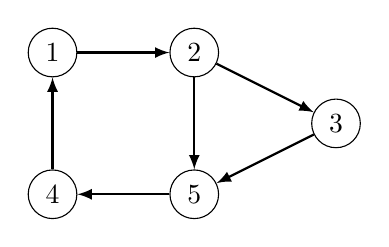
\begin{tikzpicture}[scale=0.9]
\node[draw, circle] (1) at (1,5) {$1$};
\node[draw, circle] (2) at (3,5) {$2$};
\node[draw, circle] (3) at (5,4) {$3$};
\node[draw, circle] (4) at (1,3) {$4$};
\node[draw, circle] (5) at (3,3) {$5$};

\path[draw,thick,->,>=latex] (1) -- (2);
\path[draw,thick,->,>=latex] (2) -- (3);
\path[draw,thick,->,>=latex] (4) -- (1);
\path[draw,thick,->,>=latex] (3) -- (5);
\path[draw,thick,->,>=latex] (2) -- (5);
\path[draw,thick,->,>=latex] (5) -- (4);
\end{tikzpicture}
\end{center}
các đỉnh 1, 3 và 4 đều có bậc vào 1 và bậc ra 1,
đỉnh 2 có bậc vào 1 và bậc ra 2,
và đỉnh 5 có bậc vào 2 và bậc ra 1.
Do đó, đồ thị chứa một đường đi Euler
từ đỉnh 2 đến đỉnh 5:
\begin{center}
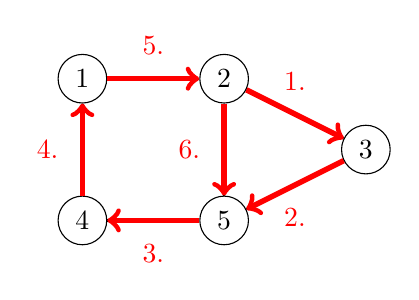
\begin{tikzpicture}[scale=0.9]
\node[draw, circle] (1) at (1,5) {$1$};
\node[draw, circle] (2) at (3,5) {$2$};
\node[draw, circle] (3) at (5,4) {$3$};
\node[draw, circle] (4) at (1,3) {$4$};
\node[draw, circle] (5) at (3,3) {$5$};

\path[draw,thick,-] (1) -- (2);
\path[draw,thick,-] (2) -- (3);
\path[draw,thick,-] (1) -- (4);
\path[draw,thick,-] (3) -- (5);
\path[draw,thick,-] (2) -- (5);
\path[draw,thick,-] (4) -- (5);

\path[draw=red,thick,->,line width=2pt] (2) -- node[font=\small,label={[red]north:1.}] {} (3);
\path[draw=red,thick,->,line width=2pt] (3) -- node[font=\small,label={[red]south:2.}] {} (5);
\path[draw=red,thick,->,line width=2pt] (5) -- node[font=\small,label={[red]south:3.}] {} (4);
\path[draw=red,thick,->,line width=2pt] (4) -- node[font=\small,label={[red]left:4.}] {} (1);
\path[draw=red,thick,->,line width=2pt] (1) -- node[font=\small,label={[red]north:5.}] {} (2);
\path[draw=red,thick,->,line width=2pt] (2) -- node[font=\small,label={[red]left:6.}] {} (5);
\end{tikzpicture}
\end{center}

\subsubsection{Thuật toán của Hierholzer}

\index{Hierholzer's algorithm}
\index{thuật toán của Hierholzer}

\key{Thuật toán của Hierholzer}\footnote{Thuật toán được công bố
vào năm 1873 sau khi Hierholzer qua đời \cite{hie73}.} là một phương pháp
hiệu quả để xây dựng
một chu trình Euler.
Thuật toán bao gồm nhiều vòng,
mỗi vòng thêm các cạnh mới vào chu trình.
Tất nhiên, chúng ta giả định rằng đồ thị chứa
một chu trình Euler; nếu không thì thuật toán của Hierholzer
không thể tìm thấy nó.

Đầu tiên, thuật toán xây dựng một chu trình chứa
một số (không nhất thiết là tất cả) các cạnh của đồ thị.
Sau đó, thuật toán mở rộng chu trình
từng bước bằng cách thêm các chu trình con vào nó.
Quá trình tiếp tục cho đến khi tất cả các cạnh đã được thêm
vào chu trình.

Thuật toán mở rộng chu trình bằng cách luôn tìm
một đỉnh $x$ thuộc chu trình nhưng có
một cạnh đi ra không được bao gồm trong chu trình.
Thuật toán xây dựng một đường đi mới từ đỉnh $x$
chỉ chứa các cạnh chưa có trong chu trình.
Sớm hay muộn,
đường đi sẽ quay trở lại đỉnh $x$,
tạo ra một chu trình con.

Nếu đồ thị chỉ chứa một đường đi Euler,
chúng ta vẫn có thể sử dụng thuật toán của Hierholzer
để tìm nó bằng cách thêm một cạnh phụ vào đồ thị
và loại bỏ cạnh đó sau khi chu trình
đã được xây dựng.
Ví dụ, trong một đồ thị vô hướng,
chúng ta thêm cạnh phụ giữa hai
đỉnh bậc lẻ.

Tiếp theo chúng ta sẽ xem thuật toán của Hierholzer
xây dựng một chu trình Euler cho một đồ thị vô hướng như thế nào.

\subsubsection{Ví dụ}

\begin{samepage}
Hãy xem xét đồ thị sau:
\begin{center}
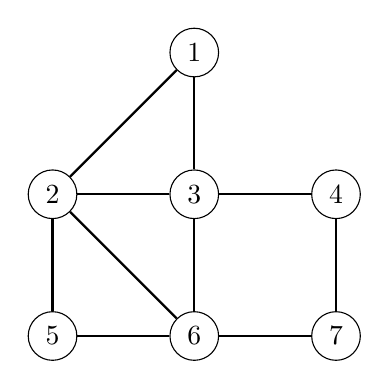
\begin{tikzpicture}[scale=0.9]
\node[draw, circle] (1) at (3,5) {$1$};
\node[draw, circle] (2) at (1,3) {$2$};
\node[draw, circle] (3) at (3,3) {$3$};
\node[draw, circle] (4) at (5,3) {$4$};
\node[draw, circle] (5) at (1,1) {$5$};
\node[draw, circle] (6) at (3,1) {$6$};
\node[draw, circle] (7) at (5,1) {$7$};

\path[draw,thick,-] (1) -- (2);
\path[draw,thick,-] (1) -- (3);
\path[draw,thick,-] (2) -- (3);
\path[draw,thick,-] (2) -- (5);
\path[draw,thick,-] (2) -- (6);
\path[draw,thick,-] (3) -- (4);
\path[draw,thick,-] (3) -- (6);
\path[draw,thick,-] (4) -- (7);
\path[draw,thick,-] (5) -- (6);
\path[draw,thick,-] (6) -- (7);
\end{tikzpicture}
\end{center}
\end{samepage}

\begin{samepage}
Giả sử rằng thuật toán đầu tiên tạo ra một chu trình
bắt đầu tại đỉnh 1.
Một chu trình có thể là
$1 \rightarrow 2 \rightarrow 3 \rightarrow 1$:
\begin{center}
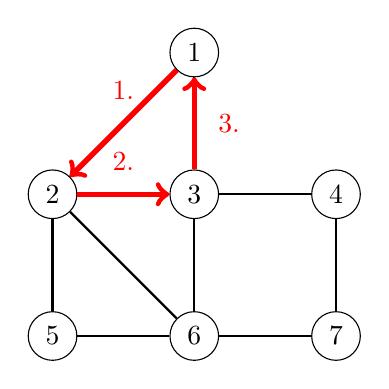
\begin{tikzpicture}[scale=0.9]
\node[draw, circle] (1) at (3,5) {$1$};
\node[draw, circle] (2) at (1,3) {$2$};
\node[draw, circle] (3) at (3,3) {$3$};
\node[draw, circle] (4) at (5,3) {$4$};
\node[draw, circle] (5) at (1,1) {$5$};
\node[draw, circle] (6) at (3,1) {$6$};
\node[draw, circle] (7) at (5,1) {$7$};

\path[draw,thick,-] (1) -- (2);
\path[draw,thick,-] (1) -- (3);
\path[draw,thick,-] (2) -- (3);
\path[draw,thick,-] (2) -- (5);
\path[draw,thick,-] (2) -- (6);
\path[draw,thick,-] (3) -- (4);
\path[draw,thick,-] (3) -- (6);
\path[draw,thick,-] (4) -- (7);
\path[draw,thick,-] (5) -- (6);
\path[draw,thick,-] (6) -- (7);

\path[draw=red,thick,->,line width=2pt] (1) -- node[font=\small,label={[red]north:1.}] {} (2);
\path[draw=red,thick,->,line width=2pt] (2) -- node[font=\small,label={[red]north:2.}] {} (3);
\path[draw=red,thick,->,line width=2pt] (3) -- node[font=\small,label={[red]east:3.}] {} (1);
\end{tikzpicture}
\end{center}
\end{samepage}
Sau đó, thuật toán thêm
chu trình con
$2 \rightarrow 5 \rightarrow 6 \rightarrow 2$
vào chu trình:
\begin{center}
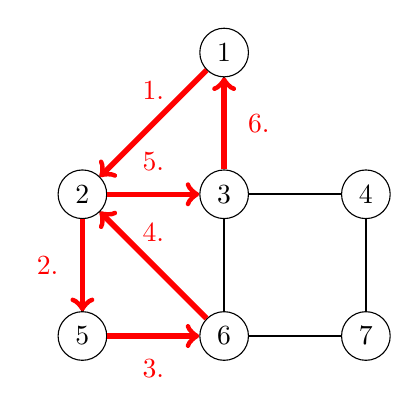
\begin{tikzpicture}[scale=0.9]
\node[draw, circle] (1) at (3,5) {$1$};
\node[draw, circle] (2) at (1,3) {$2$};
\node[draw, circle] (3) at (3,3) {$3$};
\node[draw, circle] (4) at (5,3) {$4$};
\node[draw, circle] (5) at (1,1) {$5$};
\node[draw, circle] (6) at (3,1) {$6$};
\node[draw, circle] (7) at (5,1) {$7$};

\path[draw,thick,-] (1) -- (2);
\path[draw,thick,-] (1) -- (3);
\path[draw,thick,-] (2) -- (3);
\path[draw,thick,-] (2) -- (5);
\path[draw,thick,-] (2) -- (6);
\path[draw,thick,-] (3) -- (4);
\path[draw,thick,-] (3) -- (6);
\path[draw,thick,-] (4) -- (7);
\path[draw,thick,-] (5) -- (6);
\path[draw,thick,-] (6) -- (7);

\path[draw=red,thick,->,line width=2pt] (1) -- node[font=\small,label={[red]north:1.}] {} (2);
\path[draw=red,thick,->,line width=2pt] (2) -- node[font=\small,label={[red]west:2.}] {} (5);
\path[draw=red,thick,->,line width=2pt] (5) -- node[font=\small,label={[red]south:3.}] {} (6);
\path[draw=red,thick,->,line width=2pt] (6) -- node[font=\small,label={[red]north:4.}] {} (2);
\path[draw=red,thick,->,line width=2pt] (2) -- node[font=\small,label={[red]north:5.}] {} (3);
\path[draw=red,thick,->,line width=2pt] (3) -- node[font=\small,label={[red]east:6.}] {} (1);
\end{tikzpicture}
\end{center}
Cuối cùng, thuật toán thêm chu trình con
$6 \rightarrow 3 \rightarrow 4 \rightarrow 7 \rightarrow 6$
vào chu trình:
\begin{center}
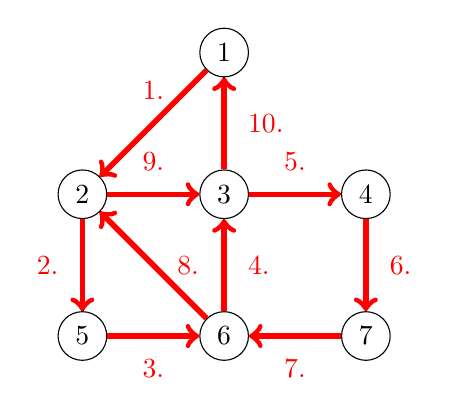
\begin{tikzpicture}[scale=0.9]
\node[draw, circle] (1) at (3,5) {$1$};
\node[draw, circle] (2) at (1,3) {$2$};
\node[draw, circle] (3) at (3,3) {$3$};
\node[draw, circle] (4) at (5,3) {$4$};
\node[draw, circle] (5) at (1,1) {$5$};
\node[draw, circle] (6) at (3,1) {$6$};
\node[draw, circle] (7) at (5,1) {$7$};

\path[draw,thick,-] (1) -- (2);
\path[draw,thick,-] (1) -- (3);
\path[draw,thick,-] (2) -- (3);
\path[draw,thick,-] (2) -- (5);
\path[draw,thick,-] (2) -- (6);
\path[draw,thick,-] (3) -- (4);
\path[draw,thick,-] (3) -- (6);
\path[draw,thick,-] (4) -- (7);
\path[draw,thick,-] (5) -- (6);
\path[draw,thick,-] (6) -- (7);

\path[draw=red,thick,->,line width=2pt] (1) -- node[font=\small,label={[red]north:1.}] {} (2);
\path[draw=red,thick,->,line width=2pt] (2) -- node[font=\small,label={[red]west:2.}] {} (5);
\path[draw=red,thick,->,line width=2pt] (5) -- node[font=\small,label={[red]south:3.}] {} (6);
\path[draw=red,thick,->,line width=2pt] (6) -- node[font=\small,label={[red]east:4.}] {} (3);
\path[draw=red,thick,->,line width=2pt] (3) -- node[font=\small,label={[red]north:5.}] {} (4);
\path[draw=red,thick,->,line width=2pt] (4) -- node[font=\small,label={[red]east:6.}] {} (7);
\path[draw=red,thick,->,line width=2pt] (7) -- node[font=\small,label={[red]south:7.}] {} (6);
\path[draw=red,thick,->,line width=2pt] (6) -- node[font=\small,label={[red]right:8.}] {} (2);
\path[draw=red,thick,->,line width=2pt] (2) -- node[font=\small,label={[red]north:9.}] {} (3);
\path[draw=red,thick,->,line width=2pt] (3) -- node[font=\small,label={[red]east:10.}] {} (1);
\end{tikzpicture}
\end{center}
Bây giờ tất cả các cạnh đã được bao gồm trong chu trình,
vì vậy chúng ta đã xây dựng thành công một chu trình Euler.

\section{Đường đi Hamilton}

\index{Hamiltonian path}
\index{đường đi Hamilton}

Một \key{đường đi Hamilton}
%\footnote{W. R. Hamilton (1805--1865) là một nhà toán học người Ireland.}
là một đường đi
thăm mỗi đỉnh của đồ thị đúng một lần.
Ví dụ, đồ thị
\begin{center}
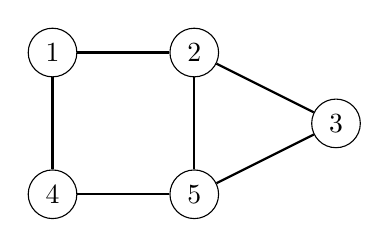
\begin{tikzpicture}[scale=0.9]
\node[draw, circle] (1) at (1,5) {$1$};
\node[draw, circle] (2) at (3,5) {$2$};
\node[draw, circle] (3) at (5,4) {$3$};
\node[draw, circle] (4) at (1,3) {$4$};
\node[draw, circle] (5) at (3,3) {$5$};

\path[draw,thick,-] (1) -- (2);
\path[draw,thick,-] (2) -- (3);
\path[draw,thick,-] (1) -- (4);
\path[draw,thick,-] (3) -- (5);
\path[draw,thick,-] (2) -- (5);
\path[draw,thick,-] (4) -- (5);
\end{tikzpicture}
\end{center}
chứa một đường đi Hamilton từ đỉnh 1 đến đỉnh 3:
\begin{center}
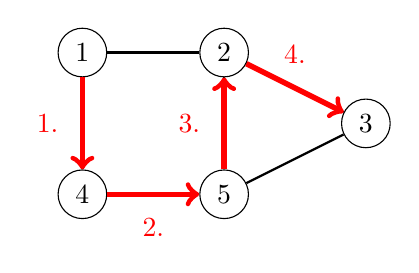
\begin{tikzpicture}[scale=0.9]
\node[draw, circle] (1) at (1,5) {$1$};
\node[draw, circle] (2) at (3,5) {$2$};
\node[draw, circle] (3) at (5,4) {$3$};
\node[draw, circle] (4) at (1,3) {$4$};
\node[draw, circle] (5) at (3,3) {$5$};

\path[draw,thick,-] (1) -- (2);
\path[draw,thick,-] (2) -- (3);
\path[draw,thick,-] (1) -- (4);
\path[draw,thick,-] (3) -- (5);
\path[draw,thick,-] (2) -- (5);
\path[draw,thick,-] (4) -- (5);

\path[draw=red,thick,->,line width=2pt] (1) -- node[font=\small,label={[red]left:1.}] {} (4);
\path[draw=red,thick,->,line width=2pt] (4) -- node[font=\small,label={[red]south:2.}] {} (5);
\path[draw=red,thick,->,line width=2pt] (5) -- node[font=\small,label={[red]left:3.}] {} (2);
\path[draw=red,thick,->,line width=2pt] (2) -- node[font=\small,label={[red]north:4.}] {} (3);
\end{tikzpicture}
\end{center}

\index{Hamiltonian circuit}
\index{chu trình Hamilton}

Nếu một đường đi Hamilton bắt đầu và kết thúc tại cùng một đỉnh,
nó được gọi là một \key{chu trình Hamilton}.
Đồ thị trên cũng có một chu trình Hamilton
bắt đầu và kết thúc tại đỉnh 1:
\begin{center}
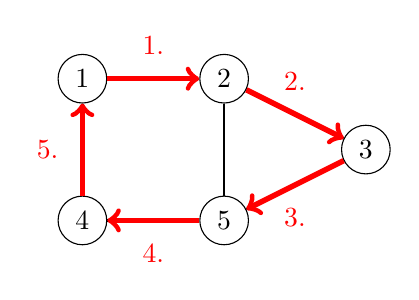
\begin{tikzpicture}[scale=0.9]
\node[draw, circle] (1) at (1,5) {$1$};
\node[draw, circle] (2) at (3,5) {$2$};
\node[draw, circle] (3) at (5,4) {$3$};
\node[draw, circle] (4) at (1,3) {$4$};
\node[draw, circle] (5) at (3,3) {$5$};

\path[draw,thick,-] (1) -- (2);
\path[draw,thick,-] (2) -- (3);
\path[draw,thick,-] (1) -- (4);
\path[draw,thick,-] (3) -- (5);
\path[draw,thick,-] (2) -- (5);
\path[draw,thick,-] (4) -- (5);

\path[draw=red,thick,->,line width=2pt] (1) -- node[font=\small,label={[red]north:1.}] {} (2);
\path[draw=red,thick,->,line width=2pt] (2) -- node[font=\small,label={[red]north:2.}] {} (3);
\path[draw=red,thick,->,line width=2pt] (3) -- node[font=\small,label={[red]south:3.}] {} (5);
\path[draw=red,thick,->,line width=2pt] (5) -- node[font=\small,label={[red]south:4.}] {} (4);
\path[draw=red,thick,->,line width=2pt] (4) -- node[font=\small,label={[red]left:5.}] {} (1);
\end{tikzpicture}
\end{center}

\subsubsection{Sự tồn tại}

Không có phương pháp hiệu quả nào được biết để kiểm tra xem một đồ thị
có chứa một đường đi Hamilton hay không, và bài toán này là NP-khó.
Tuy nhiên, trong một số trường hợp đặc biệt, chúng ta có thể chắc chắn
rằng một đồ thị chứa một đường đi Hamilton.

Một quan sát đơn giản là nếu đồ thị là đầy đủ,
tức là, có một cạnh giữa tất cả các cặp đỉnh,
nó cũng chứa một đường đi Hamilton.
Các kết quả mạnh hơn cũng đã được đạt được:

\begin{itemize}
\item
\index{Dirac's theorem}
\index{định lý Dirac}
\key{Định lý Dirac}: %\cite{dir52}
Nếu bậc của mỗi đỉnh ít nhất là $n/2$,
đồ thị chứa một đường đi Hamilton.
\item
\index{Ore's theorem}
\index{định lý Ore}
\key{Định lý Ore}: %\cite{ore60}
Nếu tổng bậc của mỗi cặp đỉnh không kề nhau
ít nhất là $n$,
đồ thị chứa một đường đi Hamilton.
\end{itemize}

Một thuộc tính chung trong các định lý này và các kết quả khác là
chúng đảm bảo sự tồn tại của một đường đi Hamilton
nếu đồ thị có \emph{một số lượng lớn} các cạnh.
Điều này có lý, bởi vì càng có nhiều cạnh trong đồ thị,
càng có nhiều khả năng để xây dựng một đường đi Hamilton.

\subsubsection{Xây dựng}

Vì không có cách hiệu quả để kiểm tra xem một đường đi Hamilton
có tồn tại hay không, rõ ràng là cũng không có phương pháp nào
để xây dựng đường đi một cách hiệu quả, bởi vì nếu không
chúng ta có thể chỉ cần thử xây dựng đường đi và xem
liệu nó có tồn tại hay không.

Một cách đơn giản để tìm kiếm một đường đi Hamilton là
sử dụng một thuật toán quay lui đi qua tất cả
các cách có thể để xây dựng đường đi.
Độ phức tạp thời gian của một thuật toán như vậy ít nhất là $O(n!)$,
bởi vì có $n!$ cách khác nhau để chọn thứ tự của $n$ đỉnh.

Một giải pháp hiệu quả hơn dựa trên quy hoạch động
(xem Chương 10.5).
Ý tưởng là tính toán các giá trị
của một hàm $\texttt{possible}(S,x)$,
trong đó $S$ là một tập hợp con các đỉnh và $x$
là một trong các đỉnh.
Hàm này cho biết liệu có một đường đi Hamilton
thăm các đỉnh của $S$ và kết thúc tại đỉnh $x$ hay không.
Có thể triển khai giải pháp này trong thời gian $O(2^n n^2)$.

\section{Chuỗi De Bruijn}

\index{De Bruijn sequence}
\index{chuỗi De Bruijn}

Một \key{chuỗi De Bruijn}
là một chuỗi chứa
mọi chuỗi có độ dài $n$
đúng một lần dưới dạng chuỗi con, cho một
bảng chữ cái cố định gồm $k$ ký tự.
Độ dài của một chuỗi như vậy là
$k^n+n-1$ ký tự.
Ví dụ, khi $n=3$ và $k=2$,
một ví dụ về chuỗi De Bruijn là
\[0001011100.\]
Các chuỗi con của chuỗi này là tất cả
các kết hợp của ba bit:
000, 001, 010, 011, 100, 101, 110 và 111.

Hóa ra mỗi chuỗi De Bruijn
tương ứng với một đường đi Euler trong một đồ thị.
Ý tưởng là xây dựng một đồ thị trong đó
mỗi đỉnh chứa một chuỗi gồm $n-1$ ký tự
và mỗi cạnh thêm một ký tự vào chuỗi.
Đồ thị sau đây tương ứng với kịch bản trên:

\begin{center}
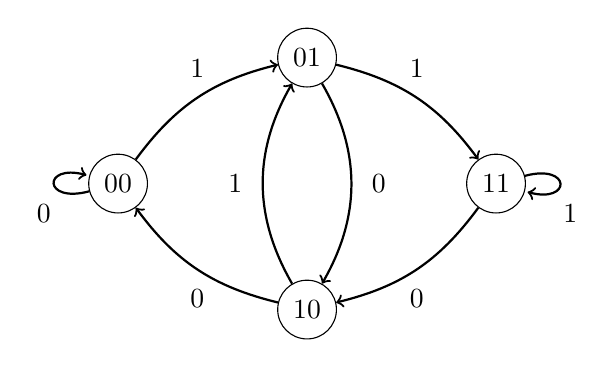
\begin{tikzpicture}[scale=0.8]
\node[draw, circle] (00) at (-3,0) {00};
\node[draw, circle] (11) at (3,0) {11};
\node[draw, circle] (01) at (0,2) {01};
\node[draw, circle] (10) at (0,-2) {10};

\path[draw,thick,->] (00) edge [bend left=20] node[font=\small,label=1] {} (01);
\path[draw,thick,->] (01) edge [bend left=20] node[font=\small,label=1] {} (11);
\path[draw,thick,->] (11) edge [bend left=20] node[font=\small,label=below:0] {} (10);
\path[draw,thick,->] (10) edge [bend left=20] node[font=\small,label=below:0] {} (00);

\path[draw,thick,->] (01) edge [bend left=30] node[font=\small,label=right:0] {} (10);
\path[draw,thick,->] (10) edge [bend left=30] node[font=\small,label=left:1] {} (01);

\path[draw,thick,-] (00) edge [loop left] node[font=\small,label=below:0] {} (00);
\path[draw,thick,-] (11) edge [loop right] node[font=\small,label=below:1] {} (11);
\end{tikzpicture}
\end{center}

Một đường đi Euler trong đồ thị này tương ứng với một chuỗi
chứa tất cả các chuỗi có độ dài $n$.
Chuỗi này chứa các ký tự của đỉnh bắt đầu
và tất cả các ký tự của các cạnh.
Đỉnh bắt đầu có $n-1$ ký tự
và có $k^n$ ký tự trong các cạnh,
vì vậy độ dài của chuỗi là $k^n+n-1$.

\section{Hành trình của quân mã}

\index{knight's tour}
\index{hành trình của quân mã}

Một \key{hành trình của quân mã} là một chuỗi các nước đi
của một quân mã trên một bàn cờ $n \times n$
theo các quy tắc của cờ vua sao cho quân mã
thăm mỗi ô đúng một lần.
Một hành trình của quân mã được gọi là một \emph{hành trình đóng}
nếu quân mã cuối cùng quay trở lại ô xuất phát và
ngược lại nó được gọi là một \emph{hành trình mở}.

Ví dụ, đây là một hành trình mở của quân mã trên bàn cờ $5 \times 5$:

\begin{center}
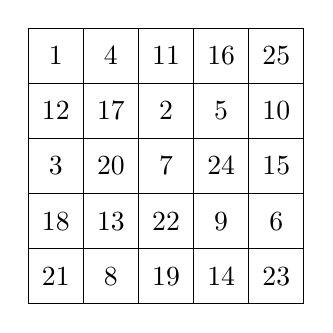
\begin{tikzpicture}[scale=0.7]
\draw (0,0) grid (5,5);
\node at (0.5,4.5) {$1$};
\node at (1.5,4.5) {$4$};
\node at (2.5,4.5) {$11$};
\node at (3.5,4.5) {$16$};
\node at (4.5,4.5) {$25$};
\node at (0.5,3.5) {$12$};
\node at (1.5,3.5) {$17$};
\node at (2.5,3.5) {$2$};
\node at (3.5,3.5) {$5$};
\node at (4.5,3.5) {$10$};
\node at (0.5,2.5) {$3$};
\node at (1.5,2.5) {$20$};
\node at (2.5,2.5) {$7$};
\node at (3.5,2.5) {$24$};
\node at (4.5,2.5) {$15$};
\node at (0.5,1.5) {$18$};
\node at (1.5,1.5) {$13$};
\node at (2.5,1.5) {$22$};
\node at (3.5,1.5) {$9$};
\node at (4.5,1.5) {$6$};
\node at (0.5,0.5) {$21$};
\node at (1.5,0.5) {$8$};
\node at (2.5,0.5) {$19$};
\node at (3.5,0.5) {$14$};
\node at (4.5,0.5) {$23$};
\end{tikzpicture}
\end{center}

Một hành trình của quân mã tương ứng với một đường đi Hamilton trong một đồ thị
có các đỉnh đại diện cho các ô của bàn cờ,
và hai đỉnh được nối với nhau bằng một cạnh nếu một quân mã
có thể di chuyển giữa các ô theo các quy tắc của cờ vua.

Một cách tự nhiên để xây dựng một hành trình của quân mã là sử dụng thuật toán quay lui.
Việc tìm kiếm có thể được thực hiện hiệu quả hơn bằng cách sử dụng
\emph{heuristic} cố gắng hướng dẫn quân mã để
một hành trình hoàn chỉnh sẽ được tìm thấy nhanh chóng.

\subsubsection{Quy tắc của Warnsdorf}

\index{heuristic}
\index{Warnsdorf's rule}
\index{quy tắc của Warnsdorf}

\key{Quy tắc của Warnsdorf} là một heuristic đơn giản và hiệu quả
để tìm một hành trình của quân mã\footnote{Heuristic này được đề xuất
trong cuốn sách của Warnsdorf \cite{war23} vào năm 1823. Cũng có
các thuật toán đa thức để tìm hành trình của quân mã
\cite{par97}, nhưng chúng phức tạp hơn.}.
Sử dụng quy tắc này, có thể xây dựng một hành trình một cách hiệu quả
ngay cả trên một bàn cờ lớn.
Ý tưởng là luôn di chuyển quân mã sao cho nó kết thúc
ở một ô mà số lượng nước đi có thể là
\emph{nhỏ nhất} có thể.

Ví dụ, trong tình huống sau, có năm
ô có thể mà quân mã có thể di chuyển đến (các ô $a \ldots e$):
\begin{center}
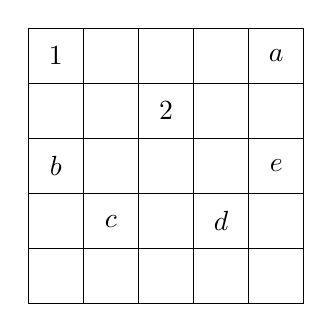
\begin{tikzpicture}[scale=0.7]
\draw (0,0) grid (5,5);
\node at (0.5,4.5) {$1$};
\node at (2.5,3.5) {$2$};
\node at (4.5,4.5) {$a$};
\node at (0.5,2.5) {$b$};
\node at (4.5,2.5) {$e$};
\node at (1.5,1.5) {$c$};
\node at (3.5,1.5) {$d$};
\end{tikzpicture}
\end{center}
Trong tình huống này, quy tắc của Warnsdorf di chuyển quân mã đến ô $a$,
bởi vì sau lựa chọn này, chỉ có một nước đi duy nhất có thể.
Các lựa chọn khác sẽ di chuyển quân mã đến các ô nơi
sẽ có ba nước đi có sẵn.


